\chapter{绪论}
\label{chap01}
近年来,随着互联网技术的发展,在线社交网络(Online Social Networks)在全世界范围内普及开来,其应用融入到了人们生活的方方面面之中。近十年来,对于在线社交网络的研究一直持续增长。在很大程度上,这归功于社交媒体以及社交服务网站的蓬勃发展。这些媒体以及网站的迅猛发展给社交网络分析(Social Network Analysis)提供了丰富的语料库与数据集。而对社交网络的研究与应用也促进了社交媒体以及社交服务网站的持续发展。在线社交网络是社会中个体集合以及个体之间连接关系所构成的网络在网络空间上的映射,即在线社交网络是真实社会在虚拟网络中的体现和拓展。在线社交网络加速了拉近了人与人之间的距离,加快了信息传播的速率,丰富了群体的结构关系。因此,在线社交网络成为了社会学、传播学、计算机科学以及系统科学等领域的研究热点。

在线社交网络是在信息网络上由用户集合以及用户之间关系所构成的社会性结构,一般而言包含三个要素:“关系结构”、“网络群体”以及“网络信息”\upcite{方滨兴2014在线社交网络分析}。三个要素之间相互关联、相互依存,其关系如图\ref{fig:threeFactors}所示。其中关系结构为网络群体的互动行为提供了基础结构以及底层平台,是社交网络的载体;网络群体推动网络信息传播,影响关系结构的演化,是社交网络的主体;网络信息的内容和传播是社交网络关键点,是群体行为的诱因和效果,同时也影响关系结构的变化,是社交网络的课题。

\begin{figure}[!ht]
    \centering
    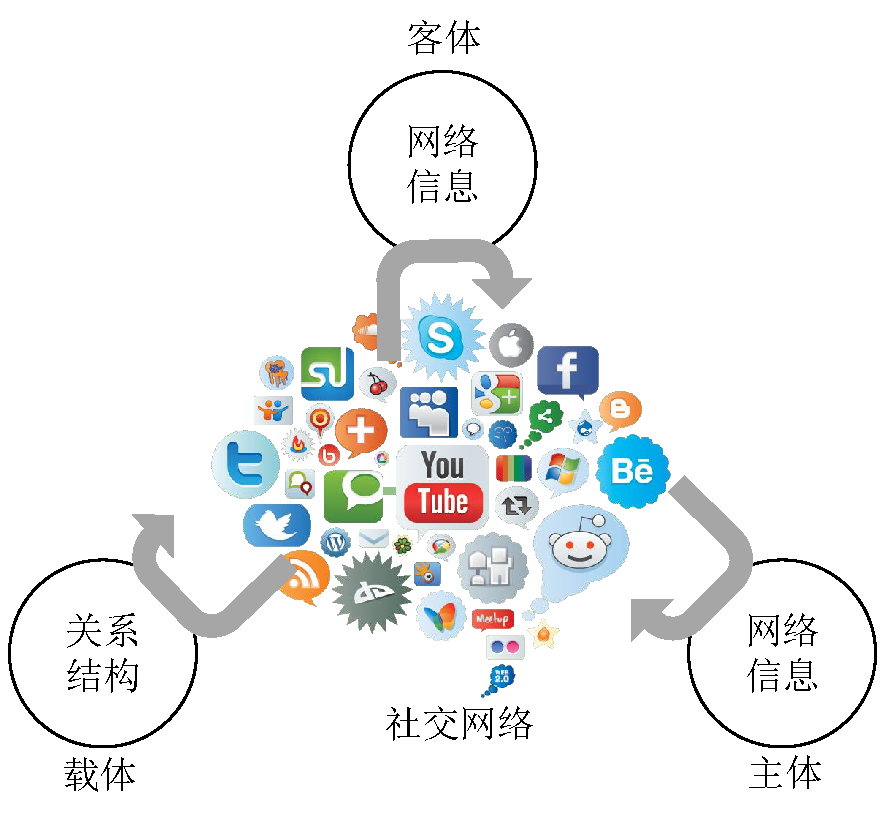
\includegraphics[width=0.5\textwidth]{threeFactors}
    \caption{在线社交网络中的关系结构、网络群体和网络信息}
    \label{fig:threeFactors}
\end{figure}

与传统的Web应用和信息媒体相比,在线社交网络具有如下的新特点:
\begin{itemize}
	\item 高速性:信息发布和接收十分便捷、迅速。社交网络中的用户可以通过手机、笔记本电脑等终端随时随地发布和接收信息,信息传递的效率高,具有高速性。
	\item 扩散性:裂变式的信息传播。社交网络中的信息一经发布,便会立刻推送到所有的关注者。信息经过转发,信息又将传播到下一批关注者。信息的传播呈现一种链式反应的几何级数扩散模式,为普通网民传播信息提供了渠道。
	\item 平等性:人人都有可能成为信息输出者。与传统信息媒体中信息发布和信息接收的非对称性相比,社交网络中的每一个参与者都有机会通过社交网络表达自己的观点,传播自己的信息,输出自身的价值观。因此,社交网络在热点事件的产生、发酵、传播等环节中扮演了重要的角色。
	\item 自发性:呈现自媒体形态、自发地形成虚拟社区。社交网络中的个体既是信息的接收者也是信息的发布者,用户会根据自身不同的关注内容与其他用户建立联系,形成网络中的虚拟社区。
\end{itemize}

这些丰富的特性让在线社交网络具有和其他信息媒体不一样的特点,同时也对信息安全提出了新的挑战。对于社交网络分析的研究,在结构、群体以及信息等方面都存在很多已有的工作。其中很多研究工作是关于网络中的信息传播、影响力、传播模型等。这些工作主要研究是否可以建立模型来解释信息的传播方式,如何在真实社交网络信息传播数据集上验证传播模型等等,这些仅仅是社交网络中信息传播研究的一些研究举例。信息传播在实际生活中有着许多应用,例如商业产品或者理念的病毒式营销、网络流量的爆发检测、寻找关键博客来获取重要的信息、寻找意见领袖或者潮流带动者以及信息的检索排序等等。

社交网络中信息传播关键技术的研究对于理解信息传播的机理有着重要的意义。本文首先在结构上进行理论研究,思考在社交网络中如何选取源节点才能使得信息传播效率更高,提出了传播效率最大化问题。然后,本文在内容方面进行分析,利用语言模型以及深度学习等技术,对普通文本信息以及数据流信息进行应用,进行了基于语义扩展和文本质量的实时个性化搜索研究和基于卷积神经网络的文本分类研究,分析不同用户的关注点,将用户所感兴趣的、高质量的信息自动地推送给用户,使得用户更加便捷地获取信息,从而推动信息的传播。最后,本文建立传播模型,对于事件的传播影响进行评估,来估测事件传播影响面的大小。本研究对于揭示信息传播的机理和规律、推动社交网络中的信息传播、发现有价值的信息以及保护信息安全起到了重要的作用。

本章首先对本文的研究背景进行阐述,第\ref{sec1:background}小节对在线社交网络中信息传播研究的发展现状进行描述,分析社交网络信息传播分析的研究意义和面临的挑战。其次,第\ref{sec1:relatedWorks}小节对本文研究的各个相关工作进行了概述和总结。然后,第\ref{sec1:inovation}小节介绍本文的主要研究内容和创新点。最后,第\ref{sec1:paperStructure}小节给出了本文的组织结构。

\section{研究背景及意义}
\label{sec1:background}
本节主要介绍本文研究的背景及其意义,对涉及到的概念进行详细的阐述,对研究所面临的挑战进行分析。首先,本节对在线社交网络进行一个概述,介绍在线社交网络的起源、定义、特点以及发展状况。其次,本节对社交网络中的信息传播进行介绍,详细地描述信息传播的特点及其所涉及到的因素。然后,本节对本文的研究的意义进行总结。最后,本节分析了研究所面临的挑战。
\subsection{在线社交网络概述}
\label{subsec1:introduction}
从人类诞生以来,就过着群居的生活,一同劳作、交流以及分享,从而形成了社会。随着人类文明的发展和社会的进步,人与人之间的关系进一步的深入和加强,社会关系由简单的血缘关系向朋友关系、雇佣关系以及社交关系发展。而人与人之间由生活、工作、学习、娱乐等等社会交互而形成了某种稳定的关系,这一系列的关系将社会个体结合成了一个巨大的网络,这即是社交网络。如同Linton Freeman所说的那样,我们都被一个无形的网络连接在一起\upcite{freeman2004development}。

社交网络(Social Network)在维基百科中被定义为由社会个体(例如个人或者机构等)、社会个体间的二元关系以及社会个体之间的社交互动组成的社会结构\upcite{social_network}。在社交网络中,个体之间因为社交互动而形成相对稳定的关系体系,这种关系可能是亲属关系、朋友关系、同学关系,也可能是商业合作关系或者宗教信仰关系等。通过这些关系,社交网络把偶然相识的弱关系到紧密结合的强关系,以及社会中各式各样的人群串联成了一张巨大的网络。由于社交网络中存在这各种各样的社会关系,个体之间的网络结构往往是非常复杂的。而且,复杂的关系结构也会影响网络中个体之间的社交互动,进而影响到个体的社会行为。

随着工业化、城市化的进行以及移动网络的发展,社会网络化的趋势日益凸显。在2012年,Lee Rainie和Barry Wellman在其著作《网络化:新的社会操作系统》\upcite{rainie2012networked}中指出,社会网络革命、移动革命以及互联网革命将是影响人类社会发展的三大革命。随着互联网的进步,网络结构受地域性因素的影响减弱了,这使得跨地域性的线上社会关系成为了社交网络的主要形式。在现实社会中,人们相继在社交媒体平台上创建账号,将线下的社会关系扩展到了线上,并且进行了进一步的延伸,这使得在线社交网络成为了人们网络生活中不可或缺的沟通工具。

在2009年欧盟关于社会计算的研究报告中\upcite{huijboom2009key},在线社交网络主要可以分成如下的四个大类,
\begin{itemize}
	\item 即时通讯应用。这一类的应用提供一个实时的通信平台,使得人与人之间能够通过网络进行在线的交流,信息的分享等。典型的代表有MSN、QQ、飞信等,其具有双向认证与实时推送的特点。
	\item 在线社交应用。这一类的应用提供一个在线社交关系平台,人们在平台上进行社交互动以及消息的共享等。典型的代表有脸书(Facebook)、谷歌+(Google+)、人人网、QQ空间等,其具有双向认证以及非实时推送的特点。
	\item 微博类型应用。这一类的应用提供一个自媒体的信息发布平台,任何个人或者机构都能在平台上发布信息,推送给其关注者。典型的代表有推特(Twitter)、新浪微博、腾讯微博等,其具有单向认证以及实时推送的特点。
	\item 共享空间以及其他应用。这一类的应用提供一个公告发布系统,具有沟通功能,但是用户之间结合不紧密。典型的代表有BBS、论坛、博客等,其具有单向认证以及非实时推送的特点。
\end{itemize}

社交网络是Web 2.0时代的具有代表性的应用,具备Web 2.0时代交互性、主动性的特点,众多社交软件应用随着技术的更新而蓬勃发展。中国流行的即时通信软件“腾讯QQ”诞生于1999年,在2016年的月活跃账户数达到8.77亿,其中智能终端月活跃账户达到6.47亿\upcite{tencentReport2016}。腾讯在2011年推出的一个为智能终端提供即时通讯服务的软件“微信”在当今已经成为了新时代移动端即时通讯的领军,微信和WeChat(微信的海外版)在2016年的合并月活跃账户数达到8.46亿\upcite{tencentReport2016}。
\subsection{社交网络信息传播}
\label{subsec1:informationDiffusion}

\subsection{研究意义}
\label{subsec1:researchSignificance}

\subsection{面临的挑战}
\label{subsec1:challenge}

\section{相关研究工作}
\label{sec1:relatedWorks}

\section{本文的工作与创新}
\label{sec1:inovation}

\section{论文结构}
\label{sec1:paperStructure}